
\section{Categorization} \label{sec:categorization}

RQ1: What categories exist within the RBAC extension models?

\subsection{Results}


During the paper reading phase, we identify categorical themes, which are
central topic or context of the RBAC extension models. 
For example, the paper ``Privacy-aware role-based access control'' \cite{ni2010privacy} brings in the notion of privacy explicitly within the title of the paper and the name of their model. 
Some papers presented this direct pronouncement of theme of the RBAC extension models, whereas others were less obvious. 
Thus, we developed a set of guidelines to aide in determining a set of eight categories based upon observations during the paper reading phase. 
In developing these guidelines, we defined each category by a single noun-phrase descriptor.
The guidelines were as follows:

\begin{itemize}
\item Model Name - Does the name of the model classify itself?
\item Self Assessment - Do the authors of the paper directly identify a descriptor for their model within the body of the paper?
\item Repetition of Phrase - Does the body of the paper present the same phrase repeatedly when discussing their model?
\end{itemize}

The previous example paper ``Privacy-aware role-based access control'' \cite{ni2010privacy} contained ``privacy'' in
the title and in the name of the model leading to the creation of the Privacy category and the subsequent placement of the paper under that category.
By comparison, the paper ``An extended RBAC model based on granular logic'' \cite{jian2008extended} does not contain a direct categorization in the title or model name. However, in reading the body of the paper, we determined that this paper discussed RBAC extension based on context. 
We offer definitions for each of the eight observed categories based on the data extracted from the primary sources and the English definitions for each noun-phrase. 
Some category descriptors contain abbreviations in parenthesis that match the shortened name found within Table \ref{tab:categorization}.

\subsection{Definitions}

\begin{itemize}

  \item \textbf{Context}: The extension model integrates contextual information into the RBAC standard model. Context is defined as a user's current state and environment (e.g., location, time, system resources, network state, network security configuration, etc) which may affect the user's access privileges.

  \item \textbf{Constraint (Const)}: The extension model provides conditional restrictions on permissions of given roles. The constraint is either static or dynamic. For example, a doctor may modify any medical record for which the doctor is assigned as the designated primary care physician. This example describes a doctor's permission with a conditional restriction - ``only when the doctor is assigned as the designated primary care physician may modify a particular medical record''.

  \item \textbf{Organizational (Org)}: The RBAC extension model is concerned with providing mechanisms and entities that allow for RBAC across multiple organizations. Typically, users may have the same role name in different organizations, but may have different access privileges due to different local variations.
  
  \item \textbf{Privacy (Priv)}: The RBAC extension model provides entities and mechanisms to describe privacy policies, which are legal statements or documents about disclosure or management of personally identifiable information such as name, address, or data of birth.
  
  \item \textbf{Task}: The RBAC extension model provides task entities which are associated with permissions and roles. A task is a fundamental unit of a business activity. Different from core RBAC, in task-role-based access control model, roles are not directly associated with permissions. Roles are associated with tasks that are associated with permissions. For example, the employee role is associated with a task, for example, to write a report. Then, this task is associated with a permission.

  \item \textbf{Spatio-Temporal}: The RBAC extension model combines spatial (location-based) and temporal (time-based) constraints in specifying access control policies. For example, specific locations permit roles to conduct actions from 8:00 a.m. to 5:00 p.m.

  \item \textbf{Spatial}: The RBAC extension model provides spatial constraints, location-based constraints in specifying access
	control policies. For example, in organizations, locations are enforced whereas a
	specific role is permitted to conduct an action. Consider that a part-time employee works only in a specific location.
	In such cases, the part-time employee role should access required resources only when the user is in that location. 
	Spatial constraints can integrate with roles, user-role assignments, or role-permission assignments. 

  \item \textbf{Temporal (Temp)}:  The RBAC extension model provides temporal constraints, time-based constraints in specifying access
	control policies. For example, in organizations, periodic temporal durations are enforced whereas a
	specific role is permitted to conduct an action. Consider that a part-time employee works only from 9:00 a.m. to 3:00 p.m.
	In such cases, the part-time employee role should be allowed to access required resources during the interval. 
	Temporal constraints can integrate with roles, user-role assignments, or role-permission assignments.   
	
\end{itemize}

\begin{figure}[ht]
    \centering
        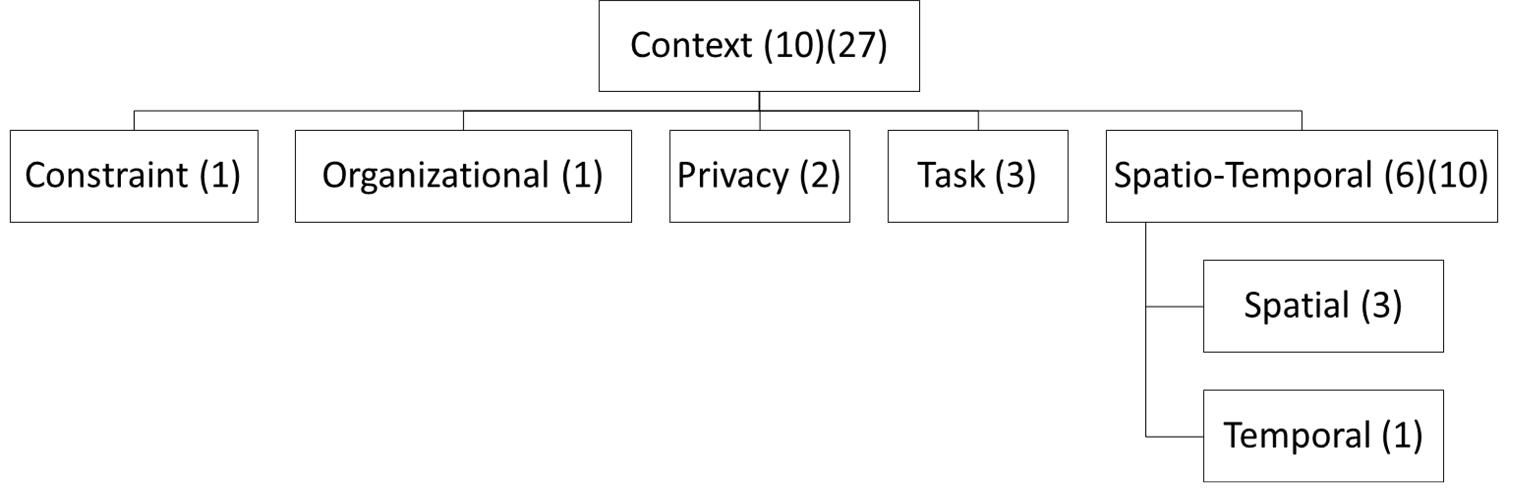
\includegraphics[width=4.0in]{sections/category_structrure.png}
\vspace{-0.2 in}
    \caption{\label{fig:category_structrure}Structure of categories within the RBAC extension models.}
\end{figure}

\subsection{Analysis and Discussion}

The 27 primary sources produced a set of eight hierarchical categories. Table \ref{tab:categorization} summarizes each primary source under their designated category and furthermore, displays the perceived hierarchy of the categories. Figure~\ref{fig:category_structrure} shows the hierarchy structure among categories. The Constraint, Organizational, Privacy, Task, and Spatial and Temporal categories can be special cases of the Context category. The Spatio-Temporal category subsumes Spatial and Temporal categories. The Spatial and Temporal categories were treated as subsets of the broader category of Spatio-Temporal since this category encompasses them individually and the Spatio-Temporal category contained more primary sources that the Spatial or Temporal categories alone.

When looking across all categories, we noted that each category added domain specific features on top of the RBAC Reference Model.
These domain specific features were under the surface these features adding contextual relationships between the core user, permission and role entities.  Thus, we
concluded that all categories stemmed from the context category, of which some primary sources were already deemed direct members.  

For example, in the case of the Privacy category, the models added entities such as purpose binding to represent within the model data collected for one purpose should not be used for another purpose without user consent {\cite{ni2010privacy}. 
While the new entity provided by the Privacy based models is inspired by domains such as healthcare where privacy is of legal concern, the underlying mechanism that drives purpose binding is providing context around making an access control decision. 
The system must take into account not just a static set of permissions a user has through their roles, but also the context of the data being accessed as that data relates to privacy policy. 
In the spatio-temporal models, a users location and the time of day are two factors that can be taken into account when activating a role or verifying a permission.  
The concepts of location and time are properties of the user and place specific contexts around the role and permission entities.

\greybox{We found eight categories that exist within the RBAC extension models: Constraint, Context, 
Organization, Privacy, Task, Spatio-Temporal, Spatial and Temporal. We further found that the other
seven categories fall under the category of Context.}
